%************************************************
\chapter{LLVM}\label{ch:LLVM}
%************************************************

The Low Level Virtual Machine (LLVM)is a compiler framework developped by Lattner and Adve\todo{Citer llvm}. The main idea is that LLVM works on an intermediate language, called LLVM-IR. This language is between assembly and high level language : human-readable but close to architecture. The framework operates at compile time, at link time and at run time using analysis and transformations passes. LLVM can generate executable for different architectures like x86, x86-64, ARM and also for parallel architectures with the NVPTX backend. The LLVM pipeline can process a variety of programming languages, for instance C/C++, FORTRAN, Ruby, Python. 

\section{LLVM Architecture and Pipeline}
LLVM is not a single-block application but a set of libraries. Each library do a single step in the LLVM pipeline. It is possible to call only one library with the command line or let the compiler work by itself. In this section, the LLVM Pipeline will be described. At each stage, the corresponding tool will be mentionned.

The LLVM pipeline, show in a simplified way in Figure~\ref{fig:Architecture}, can be schematize as follows :

\begin{figure}
\centering
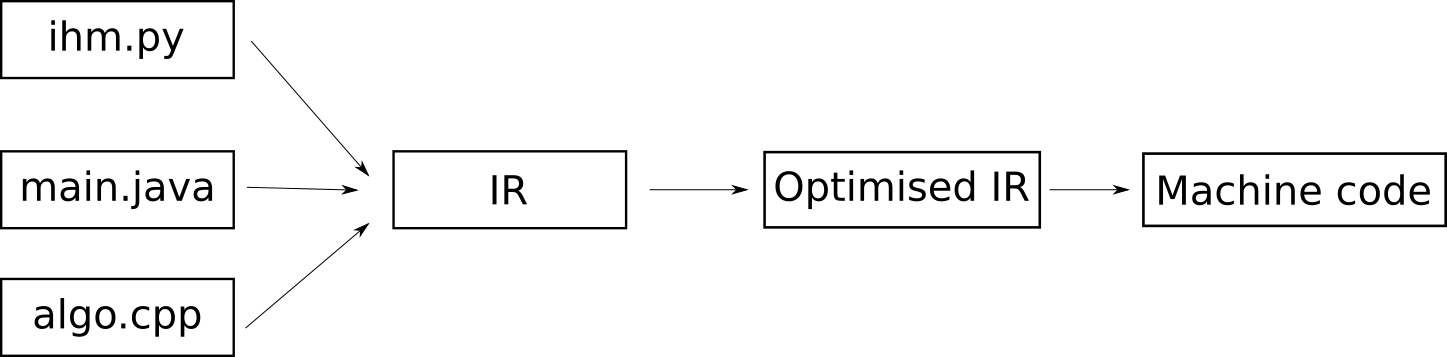
\includegraphics[scale=0.25]{gfx/LLVM/Architecture.png}
\caption{Simplified LLVM Architecture}
\label{fig:Architecture}
\end{figure}

On the left hand side, the input source file are processed by the front-ends corresponding to the language of the source code. The front-end provides to the rest of the pipeline a ll file, which is a file containing LLVM-IR. The tool use for the front end differ according to source code. For example, in case of C/C++, the tool can be clang.

These files are given to an optimiser and are optimized independently. A set of common optimisations can be performed. But the user can specify which passes to run. The tool for this stage is llvm-opt. It is possible to specify with an option to execute only some passes. For instance, to enable Polly, the "-polly" option is needed to allow polyhedral optimizations.

After this stage, llvm-link links every ll files into a single module.

This module can be optimized again with llvm-opt. All source code are merged in one module, so it is possible to optimise C++ code that is inside a python method. 

Once the ll file is optimized, an object file is generated using llvm-llc and llvm-mc. During these steps, optimizations for specific architectures can be done. For instance, generating instructions that handle array will not be generated in the same manner on a x86-64 processor and on a GPU.

\section{LLVM IR}
One of the best concept of LLVM is the intermediate representation. This language is used throughout all the LLVM Pipeline. Every compiler that uses LLVM as backend to optimize the code transforms the source code to a LLVM-IR version. LLVM-IR is independant of the target architecture, typed and assume an infinite number of registers. Each register is written only once so that the operations are in Static Single Assignement form (SSA). 

A LLVM-IR file is just a list of instructions. Passes can add, remove or modify instructions. For instance, it is possible to add malloc and free calls with the following methods :
\begin{lstlisting}[frame=single]
CreateMalloc (Instruction *InsertBefore, Type *IntPtrTy, Type *AllocTy, Value *AllocSize, Value *ArraySize=nullptr, Function *MallocF=nullptr, const Twine &Name="")
CreateFree (Value *Source, Instruction *InsertBefore)
\end{lstlisting}

In this thesis, some examples will be written in LLVM-IR for the sake of simplicity. If the reader has some troubles to understand the code, a full definition can be found \href{https://llvm.org/docs/LangRef.html}{here}.

\section{Passes}
LLVM works with a mechanism of passes. Passes perform transformations and optimizations on the code. They also make analysis that will be used by other passes. A pass can depends on others passes. For instance, a pass that get rid of dependencies will depend on the pass that computes these dependencies.

Each pass is register to a pass manager. It is possible to enable a pass in the opt command line by adding -<name of the pass>. 

There are multiples types of passes in LLVM, depending on which kind of object it iterate on. Here are the main one :
\begin{itemize}
\item ModulePass
\item FunctionPass
\item LoopPass
\item RegionPass
\item BasicBlockPass
\end{itemize}
A basic block is a single entry single exit section of code.
